\documentclass[11pt, a4paper, twoside, openright]{article} %draft

\usepackage{graphicx,color}
\usepackage{amssymb, amsmath, array}
\usepackage{hyperref}
\usepackage{enumitem}
\usepackage{lscape}
\usepackage{pdfpages}

\begin{document}

% Example of title page for the projects carried out within DEDIS
% Copied from lasec 

% Simply include it in your mastex tex file: 
%        % Example of title page for the projects carried out within DEDIS
% Copied from lasec 

% Simply include it in your mastex tex file: 
%        % Example of title page for the projects carried out within DEDIS
% Copied from lasec 

% Simply include it in your mastex tex file: 
%        \input{cover}


% Updated October 2016


\newcommand{\logoepfl}[0]{
  \begin{center}
    
\includegraphics[width=4cm]{logo_epfl_coul.eps}
  \end{center}
  \vspace{0.3cm}
  \hrule
}
\newcommand{\project}[1]{
  \begin{center}
    \large{#1}
  \end{center}
  \vspace{1cm}
}
\newcommand{\department}[1]{
  \begin{center}
    \large{#1}
  \end{center}
}
\newcommand{\lab}[1]{
  \begin{center}
    \large{#1}
  \end{center}
}
\newcommand{\supervisor}[3]{
  \begin{center}
    \begin{normalsize}{
        \bf #1}\\#2\\#3
    \end{normalsize}
  \end{center}
}
\renewcommand{\author}[1]{
  \begin{center}
    \Large{#1}
  \end{center}
  \vspace{0.5cm}
}
\renewcommand{\title}[1]{
  \vspace{3cm}
  \begin{center}
    \huge{#1}
  \end{center}
  \vspace{1.7cm}
}
\renewcommand{\date}[2]{
  \begin{center}
    \normalsize{#1 #2}
  \end{center}
  \vspace{0.5cm}
}


\thispagestyle{empty}


% begin title page
  \logoepfl
  
  \title{Explore cross-platform mobile platforms}
  
  \author{Louis-Maxence Garret}
  \department{School of Computer and Communication Sciences}
  \lab{Decentralized and Distributed Systems lab}
  \project{Master Optional Project}
  
  \date{January}{2019}

  \begin{center}
    \begin{tabular}{cc}
      \begin{tabular}{p{4.0cm}}
        \supervisor{Responsible}{Prof. Bryan Ford}{EPFL / DEDIS}
      \end{tabular}&
      \begin{tabular}{p{4.0cm}}
        \supervisor{Supervisor}{Linus Gasser}{EPFL / DEDIS}
      \end{tabular}
    \end{tabular}
  \end{center}

% end title page




% Updated October 2016


\newcommand{\logoepfl}[0]{
  \begin{center}
    
\includegraphics[width=4cm]{logo_epfl_coul.eps}
  \end{center}
  \vspace{0.3cm}
  \hrule
}
\newcommand{\project}[1]{
  \begin{center}
    \large{#1}
  \end{center}
  \vspace{1cm}
}
\newcommand{\department}[1]{
  \begin{center}
    \large{#1}
  \end{center}
}
\newcommand{\lab}[1]{
  \begin{center}
    \large{#1}
  \end{center}
}
\newcommand{\supervisor}[3]{
  \begin{center}
    \begin{normalsize}{
        \bf #1}\\#2\\#3
    \end{normalsize}
  \end{center}
}
\renewcommand{\author}[1]{
  \begin{center}
    \Large{#1}
  \end{center}
  \vspace{0.5cm}
}
\renewcommand{\title}[1]{
  \vspace{3cm}
  \begin{center}
    \huge{#1}
  \end{center}
  \vspace{1.7cm}
}
\renewcommand{\date}[2]{
  \begin{center}
    \normalsize{#1 #2}
  \end{center}
  \vspace{0.5cm}
}


\thispagestyle{empty}


% begin title page
  \logoepfl
  
  \title{Explore cross-platform mobile platforms}
  
  \author{Louis-Maxence Garret}
  \department{School of Computer and Communication Sciences}
  \lab{Decentralized and Distributed Systems lab}
  \project{Master Optional Project}
  
  \date{January}{2019}

  \begin{center}
    \begin{tabular}{cc}
      \begin{tabular}{p{4.0cm}}
        \supervisor{Responsible}{Prof. Bryan Ford}{EPFL / DEDIS}
      \end{tabular}&
      \begin{tabular}{p{4.0cm}}
        \supervisor{Supervisor}{Linus Gasser}{EPFL / DEDIS}
      \end{tabular}
    \end{tabular}
  \end{center}

% end title page




% Updated October 2016


\newcommand{\logoepfl}[0]{
  \begin{center}
    
\includegraphics[width=4cm]{logo_epfl_coul.eps}
  \end{center}
  \vspace{0.3cm}
  \hrule
}
\newcommand{\project}[1]{
  \begin{center}
    \large{#1}
  \end{center}
  \vspace{1cm}
}
\newcommand{\department}[1]{
  \begin{center}
    \large{#1}
  \end{center}
}
\newcommand{\lab}[1]{
  \begin{center}
    \large{#1}
  \end{center}
}
\newcommand{\supervisor}[3]{
  \begin{center}
    \begin{normalsize}{
        \bf #1}\\#2\\#3
    \end{normalsize}
  \end{center}
}
\renewcommand{\author}[1]{
  \begin{center}
    \Large{#1}
  \end{center}
  \vspace{0.5cm}
}
\renewcommand{\title}[1]{
  \vspace{3cm}
  \begin{center}
    \huge{#1}
  \end{center}
  \vspace{1.7cm}
}
\renewcommand{\date}[2]{
  \begin{center}
    \normalsize{#1 #2}
  \end{center}
  \vspace{0.5cm}
}


\thispagestyle{empty}


% begin title page
  \logoepfl
  
  \title{Explore cross-platform mobile platforms}
  
  \author{Louis-Maxence Garret}
  \department{School of Computer and Communication Sciences}
  \lab{Decentralized and Distributed Systems lab}
  \project{Master Optional Project}
  
  \date{January}{2019}

  \begin{center}
    \begin{tabular}{cc}
      \begin{tabular}{p{4.0cm}}
        \supervisor{Responsible}{Prof. Bryan Ford}{EPFL / DEDIS}
      \end{tabular}&
      \begin{tabular}{p{4.0cm}}
        \supervisor{Supervisor}{Linus Gasser}{EPFL / DEDIS}
      \end{tabular}
    \end{tabular}
  \end{center}

% end title page



\newpage
\thispagestyle{empty}
\tableofcontents{\protect\thispagestyle{empty}
\newpage
        
% Start page count
\setcounter{page}{1}

\section{Introduction}

%%% Motivation

Upon buying a second-hand car, in most cases, consumers wonder whether that particular car has been stolen in the past or holds some hidden flaws. Frauds are very common when it comes to previously owned vehicles and some examples include tampering with the readings of odometers, hiding maintenance details as well as the history of accidents.\\
\newline
This problem in the automotive industry costs the consumers, car dealers, manufacturers, insurance and leasing companies approximately between 5.6 and 9.6 billion euros per year in Europe \cite{Costs}.
Thus, the question that persists is how to fight these criminal deceptions and establish trust among the above-mentioned entities.\\
\newline
Our motivation is to create a solution that allows buyers to be confident in their purchase and owners to increase the value of their car. We propose a proof of concept that includes a blockchain for keeping maintenance data of cars in form of a digital registry, where the records persist forever and are resistant to manipulation.\\
\newline
The idea is to add maintenance reports for every regular vehicle inspection, as well as for every unexpected malfunctioning or car crash. Some of the data used in these reports is generated by IoT devices that measure mileage, score of well driving and other parameters when placed on a vehicle.\\ 
\newline
This documentation is structured to offer a background information about the blockchain technology in section~\ref{Background} and then introduce an overview of the project in section~\ref{Overview}.\\
\newline
Furthermore, in section~\ref{Implementation}, we cover the implementation details of our work, including the management of access rights, creation of digital contracts for enforcing specific performance, handling the private data and also the interaction between the users and the blockchain.\\
\newline
Finally, in section~\ref{Evaluation} we test and evaluate the behaviour of our system in larger networks and with parallel transactions. We utilize visualized charts in order to draw better conclusions and then we finish our work with future possibilities for improvement.\\
\newline
In summary, this project shows how the blockchain technology can be applied in other spheres of the real world (particularly in the automotive industry), and not only in the well known financial area, with the purpose of solving trust and fraud issues.

\newpage
\section{Evaluation of cross-platform frameworks}
\subsection{App requirements}
In order to compare each framework, a list of features to be implemented in the developed applications was established: 
\begin{itemize}
	\item QR Code Reader: for the mobile apps developed at DEDIS such as popcoins, information is passed between users/devices using QR Codes. Information on one device is encoded into a JSON string, then encoded into a QR Code, read by the other device and parsed the other way around. In the case of the apps developed for this project, the passed information is simply composed of a name, a public key and an address. These allow the application to contact the specified conode (cothority node).
	\item Displaying the conode's status: once the JSON encoded information is decoded, the app has to contact the conode and get its status. This requires establishing communication with the cothority using protobuf over websockets. 
	\item Storing and retrieving information on the device: the app has to store the conode information (address and public key) into permanent memory on the device, in order to retrieve it when restarting and thus keeping track of the same conode.
	\item Schnorr's signature benchmarking: in order to be useful for the DEDIS lab, the framework must be able to perform edwards25519 operations, in a reasonable amount of time. The app has to implement a benchmark on those operations, in the form of performing 100 Schnorr's signatures and validations.
\end{itemize}


\subsection{Evaluation criteria}
Once those features are either implemented or found impossible to implement, the frameworks are evaluated on the following criteria:

\begin{itemize}
	\item Licensing: before getting into the development part, it is important to make sure that the framework tested allows distributing created applications with the wanted license. 
	
	\item Ease of integration with existing libraries: the cothority was already developed in Go, JavaScript and Java languages, however some functionalities require the development framework to support extra libraries (e.g. for edwards25519 operations or websockets). Code adaptation might be necessary in some cases to have the cothority working, and sometimes the framework might not provide libraries suitable to use with it.
	
	\item Debugging: during the development of an application, even when implementing only basic features, having access to a fully featured and functional debugger is crucial. The ease of use of debuggers, their features and their stability are evaluated.
	
	\item UI widgets and layouts: not having to reinvent the wheel for the UI of an application is of course a must-have for any mobile framework. Also, some of the UI library provided might not have adaptive designs to have the native feeling on both iOS and Android platforms.
	
	\item Deployment: this part evaluates how the deployment process goes, from building the application with its libraries, writing tests, to the installation on the device. It also covers the issues encountered on some frameworks while attempting to build the application.
	
	\item Benchmark: for each framework where it was possible, a benchmark consisting of 100 Schnorr's signatures with validation was performed. This subsection gives the benchmark's results and a further investigation in case of a gap in performances.
	
\end{itemize}

We will now discuss those criteria for each frameworks explored with this project.

\newpage
\section{NativeScript}
\label{sec:nativescript}

\begin{figure}[!htb]
	\centering
	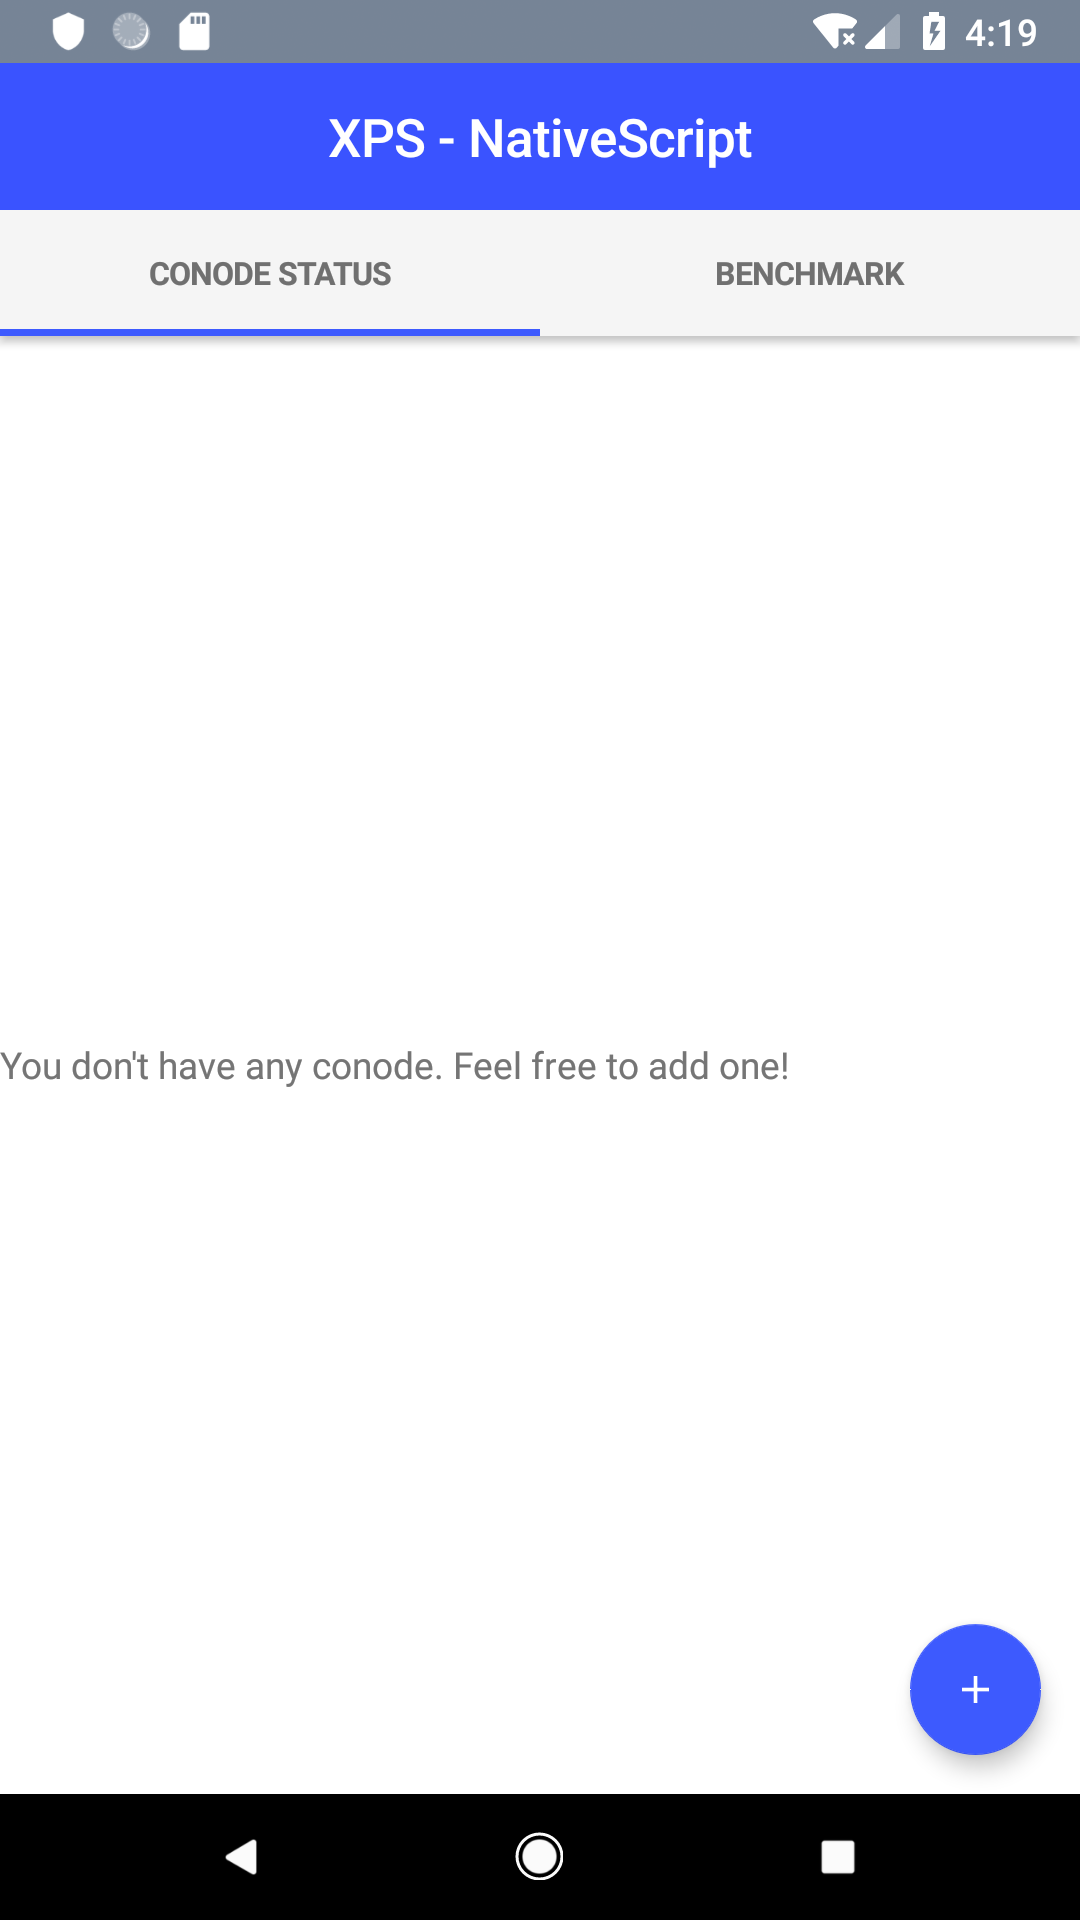
\includegraphics[width=0.35\textwidth]{img/NativeScript_layout_android.png}
	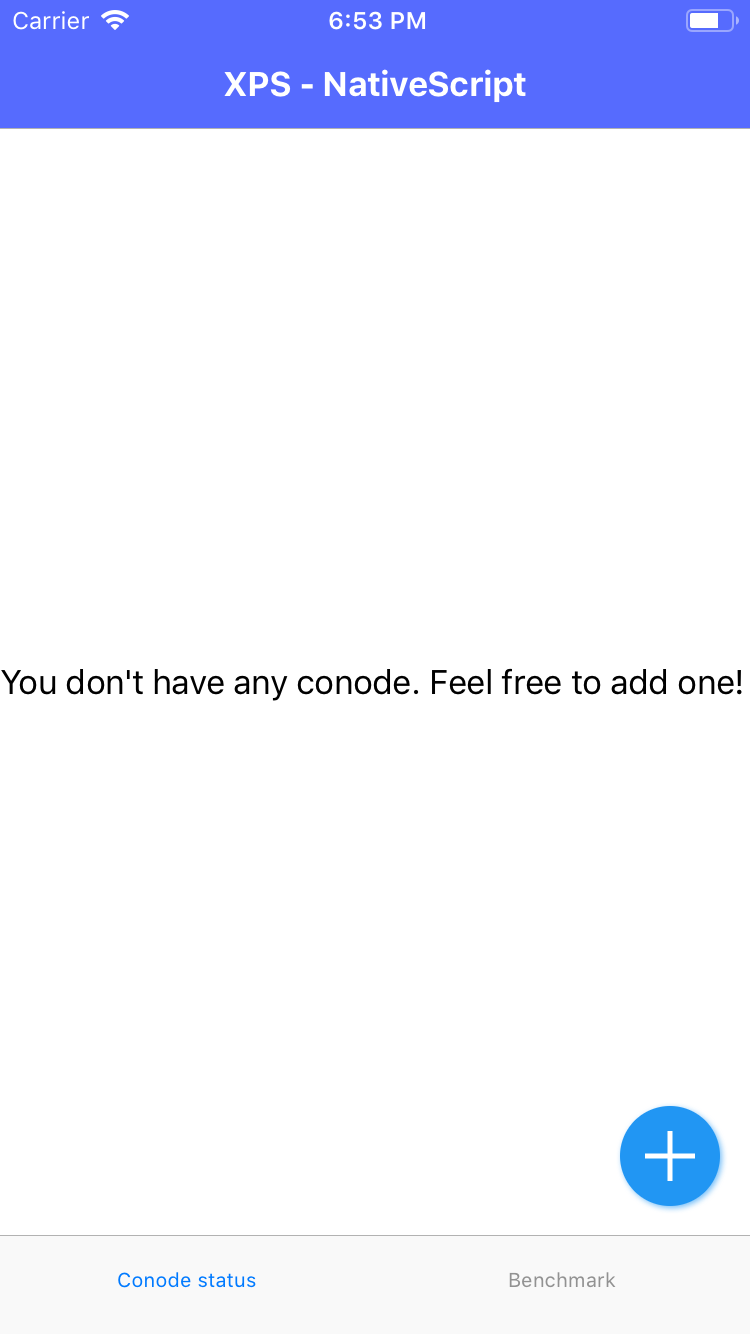
\includegraphics[width=0.35\textwidth]{img/NativeScript_layout_ios.png}
	
	\caption{NativeScript: Tab layout in Android (left) and iOS (right)}
	\label{fig:nativescript_layout_comparison}
\end{figure}

NativeScript is a free and open-source framework used to develop mobile applications for iOS and Android with Angular, Vue.js, TypeScript or JavaScript. It is developed and maintained by the Progress Software Corporation.\\
DEDIS cross platform applications are already developed using the NativeScript framework. The resulting application of this project use many code parts of the popcoins app\footnote{\url{https://github.com/dedis/popcoins}} in order to fulfil the requirements. The development process was faster than starting over with a whole different framework.\\

Before getting into details, here is a summary of what is important:
\begin{itemize}
	\item Every feature was implemented. The only issue is the benchmark running on the UI thread.
	\item Distributed under the Apache 2.0 license.
	\item Thanks to work already done using this framework, easy integration (cothority already NativeScript compatible).
	\item Debugging is complete and easy to use.
	\item Provides UI widgets and layouts necessary.
	\item Easy deployment.
	\item Cryptographic operations fast on Android, slow on iOS
\end{itemize}

Let's now evaluate this framework according to our criteria.

\subsection{Implementation}
The QR Code reader for the NativeScript app was implemented using the nativescript-barcodescanner\footnote{\url{https://github.com/EddyVerbruggen/nativescript-barcodescanner}}. It is fully functional and works as intended on both iOS and Android.

As mentioned at the beginning of part \ref{sec:nativescript}, this application was built using many code parts from the popcoin app. In particular, the cothority was already made to be NativeScript compatible. Contacting a conode via a websocket and getting its status is working as expected on this framework, on both platforms.

Using the application-settings\footnote{\url{https://docs.nativescript.org/ns-framework-modules/application-settings}} module provided natively by NativeScript, the app is able to save to memory a given string. We use it to save basic conode information JSON encoded. This module works, as expected, on both iOS and Android platforms.

Schnorr's signature and validation runs on both mobile platforms, but the benchmark does not run in background, leading to a UI freeze.

\subsection{Licensing}
NativeScript is distributed under the Apache 2.0 License\footnote{\url{https://www.nativescript.org/blog/nativescript-licensing-explained}}, which allows usage, modification, distribution, commercial use, sub-licensing. 

\subsection{Ease of integration}
As mentioned at the beginning of section \ref{sec:nativescript}, the integration of the existing JavaScript libraries to a NativeScript codebase was already done during the development of the popcoin app. No further integration was necessary here, thus the integration could be considered as easy.

\subsection{Debugging}
Thanks to the work of a non-affiliated to NativeScript developer, there exists a plugin for JetBrains IDEs (especially WebStorm in our case) that allows for an easy and complete debugging. Using the \{N\} plugin\footnote{\url{https://plugins.jetbrains.com/plugin/8588-nativescript}}, one can easily deploy an application in debug mode, set breakpoints, and explore variables and the stack as needed. Even though this plugin is non-official, it works flawlessly and makes debugging on NativeScript stable and convenient.

\subsection{UI widgets and layouts}
NativeScript UI library includes most of the necessary layouts and widgets. It features a tab layout that will adapt to have a native look depending on the platform, as shown on Fig. \ref{fig:nativescript_layout_comparison}.
It also possible to use third parties modules in order to add the wanted layouts/widgets necessary. This was the case for the floating action button, that was not provided by the NativeScript's UI library. 

\subsection{Deployment}
After patching two of the used Node.js packages, the building and deploying processes of NativeScript are usually stable.\\

NativeScript supports unit testing with JavaScript test frameworks such as Mocha\footnote{\url{https://mochajs.org/}} or Jasmine\footnote{\url{https://jasmine.github.io/}}. UI testing is done using Appium\footnote{\url{https://github.com/NativeScript/nativescript-dev-appium/}} although it is not included by default.\\

More details can be found in subsection \ref{sub:appendix_nativescript_deployment}.



\subsection{Benchmark}
The results for the benchmark (100 Schnorr's signatures and validation) are the following:
\begin{itemize}
	\item Android: 4024ms
	\item iOS: 126231ms
\end{itemize}

After some investigation, it was found that the cause of this huge difference of time to complete the 100 operations was due to the multiplication operation between a point and a scalar in the Schnorr implementation running much slower (363.3 ms) on iOS compared to Android (12.4ms). \\

\newpage
\section{React Native}

\begin{figure}[!htb]
	\centering
	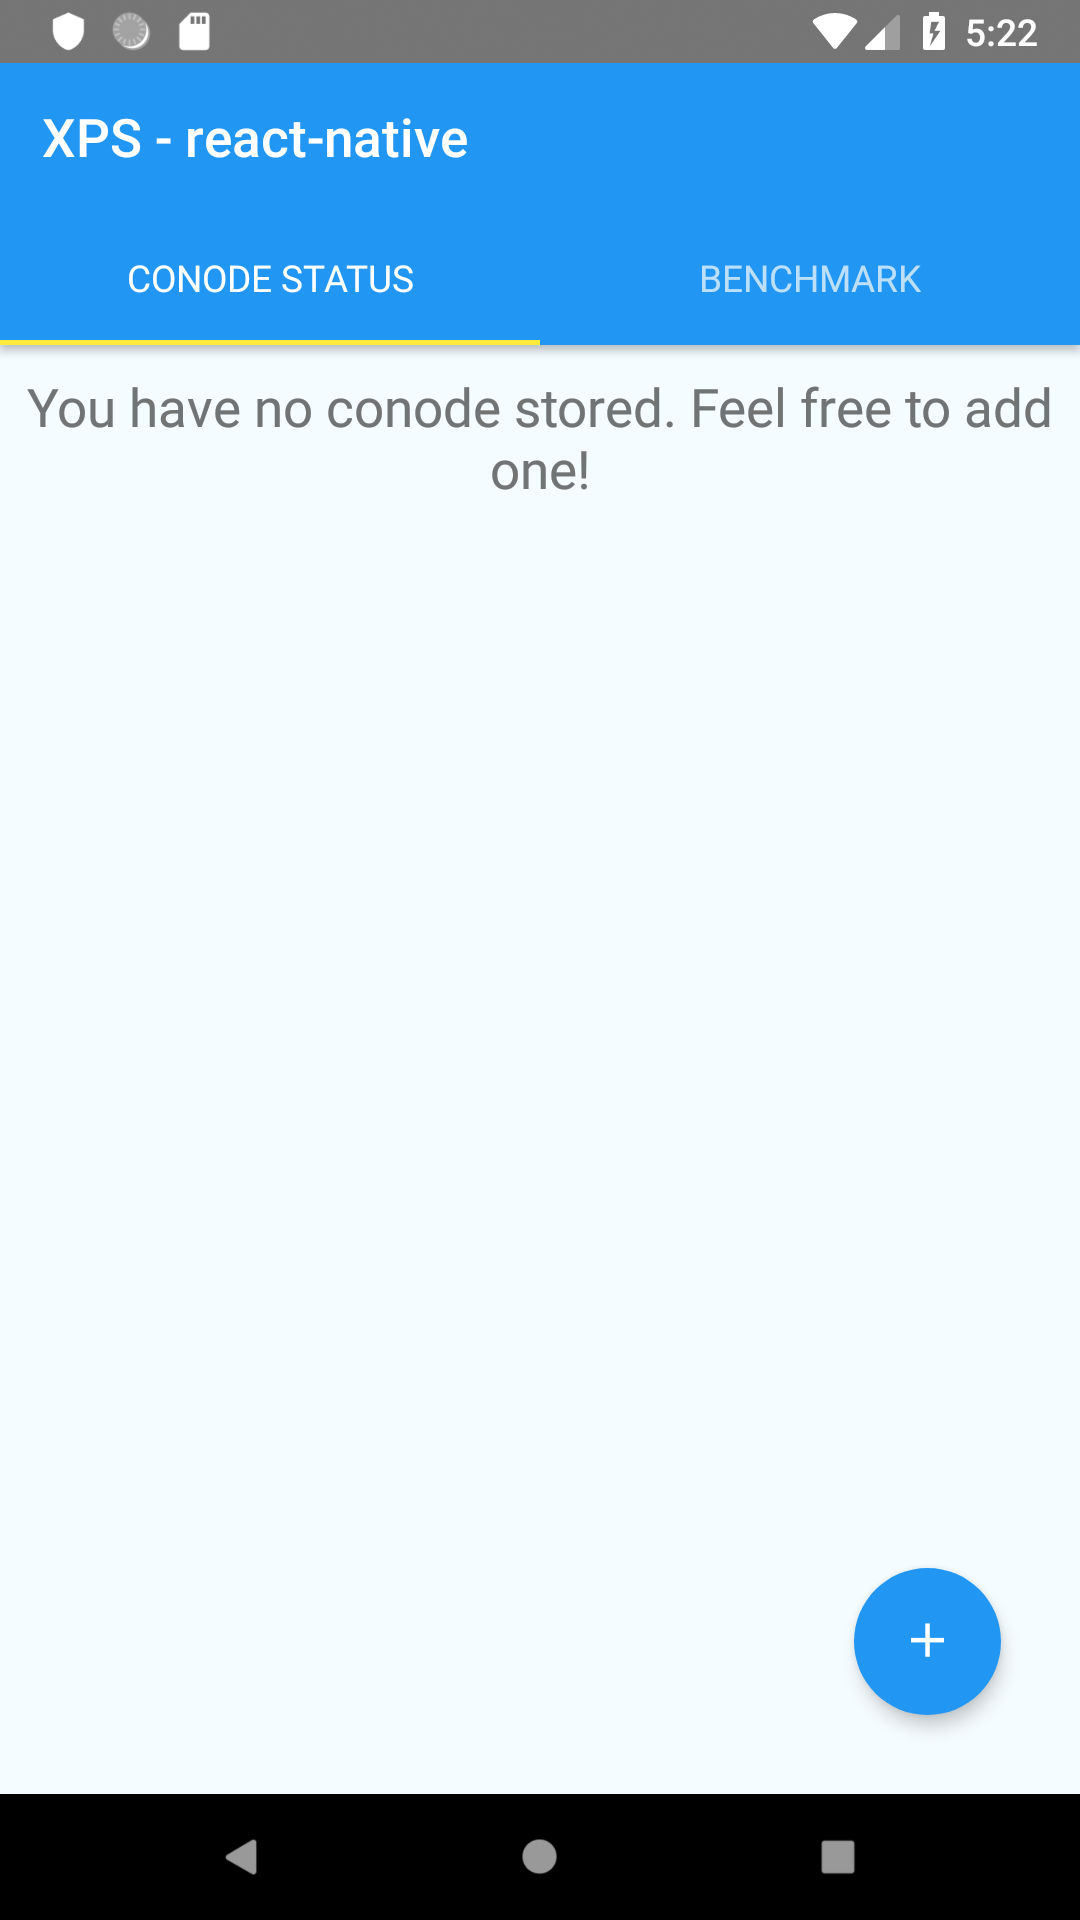
\includegraphics[width=0.35\textwidth]{img/react_layout_android.png}
	
	\caption{React Native: Tab layout on Android}
	\label{fig:react_layout}
\end{figure}

React Native is a free and open-source framework that allows developing mobile applications for iOS and Android with React (JavaScript). It is developed and maintained by Facebook.\\
As many DEDIS libraries are already written in JavaScript, React Native could be an interesting alternative to the NativeScript framework.\\

Before getting into the details, here is a summary of what is important:
\begin{itemize}
	\item It was not possible to get websockets to work in React Native, as there is no support for it and third parties packages did not work as intended.
	\item A recent update of the framework combined with Xcode 10 broke the ability to build the iOS app. This issue could not be solved even by falling back to previous software versions.
	\item React Native is distributed under the MIT license.
	\item The integration is incomplete, but most of the adaptations that do work were done easily.
	\item Debugging is not intuitive and even faulty some times.
	\item Provides UI widgets and layouts necessary.
	\item Deployment is pretty easy and Android, complicated for iOS.
	\item Schnorr signature and validation calculated at correct speed on Android, unknown on iOS.
\end{itemize}

Let's now talk about the status of the app created using this framework.

\subsection{Implementation}
The QR Code reader was implemented using the react-native-qrcode-scanner package\footnote{\url{https://github.com/moaazsidat/react-native-qrcode-scanner}} package. It works flawlessly on the iOS and Android platforms.

\label{sub:react_conode_status}
React Native has native websocket support and provides documentation\footnote{https://facebook.github.io/react-native/docs/network} about it. However, the implementation of websockets provided by React Native drops the connection unexpectedly when trying to contact a conode. The app cannot display a conode's status.

Storage was implemented using the react-native-storage\footnote{\url{https://github.com/sunnylqm/react-native-storage}} package. It has been tested to be fully functional on Android and unknown on iOS (details in appendix \ref{sub:appendix_react_deployment}).

Some adaptation of the JavaScript codebase was necessary in order to get the Schnorr's signatures and verifications working. Using the corresponding crypto libraries for React Native, the Schnorr's signatures and verifications are working on Android (and technically unknown on iOS). As for NativeScript, the benchmark does not run in the background.

\subsection{Licensing}
React Native is distributed under the MIT license\footnote{\url{http://www.reactnative.com/react-native-now-has-mit-licence/}}, which allows usage, modification, distribution, commercial use, sub-licensing.

\subsection{Ease of integration}
As React Native apps are developed in JavaScript, the cothority version edited for NativeScript was imported in the application. Some parts of the code needed to be rewritten, as the packages used with NativeScript are usually not the same as for other JavaScript frameworks. But it was usually easy to find an alternative pure JavaScript package for a given NativeScript package, and replace its usage in the code.\\
As mentioned in subsection \ref{sub:react_conode_status}, the websocket communication was rewritten to fit the React Native APIs for websocket usage, but without success. When attempting to contact a conode, the connection drops after the first exchange of messages, without reconnection.\\
The integration of the cryptographic part of the cothority library was done easily. This means that in order to adapt the existing JavaScript libraries used at DEDIS for React Native, the only true challenge to address remains the websocket issue. 


\subsection{Debugging}
\label{sub:react_debug}
Developer can debug React Native directly in WebStorm, using breakpoints and browsing the stack and variable states. Unfortunately, the debugger tool is unstable to unreliable, as detailed in appendix \ref{sub:appendix_react_debugging}.

\subsection{UI widgets and layouts}
React Native provides a greatly furnished UI library for mobile applications. Some layouts and widgets are missing but can be added through community packages.
Using the react-native-tab-view\footnote{\url{https://github.com/react-native-community/react-native-tab-view}}, it is possible to have a tab layout. However, the look and feel of it is closer to the native Android layout than the iOS one, on both mobile platforms, as shown in fig. \ref{fig:react_layout}.

\subsection{Deployment}
Deployment for Android is quite stable, but currently broken for iOS, for reasons detailed in appendix \ref{sub:appendix_react_deployment}.

Unit testing in React Native is done by using Jest\footnote{\url{https://jestjs.io/en/}}. It possible to integrate Appium tests to Jest tests\footnote{\url{https://medium.com/@7ynk3r/react-native-e2e-testing-with-appium-on-sauce-labs-8920195b8a54}} for UI testing.
\subsection{Benchmark}
\label{sub:react_benchmark}
For Android, the result of the benchmark is 18908ms. This is slower than the NativeScript Android app, but can be considered as a tolerable time for that amount of signatures. Unfortunately, the iOS version could not be benchmarked because of the build issue mentioned previously.

\newpage
\section{Flutter}

\begin{figure}[!htb]
	\centering
	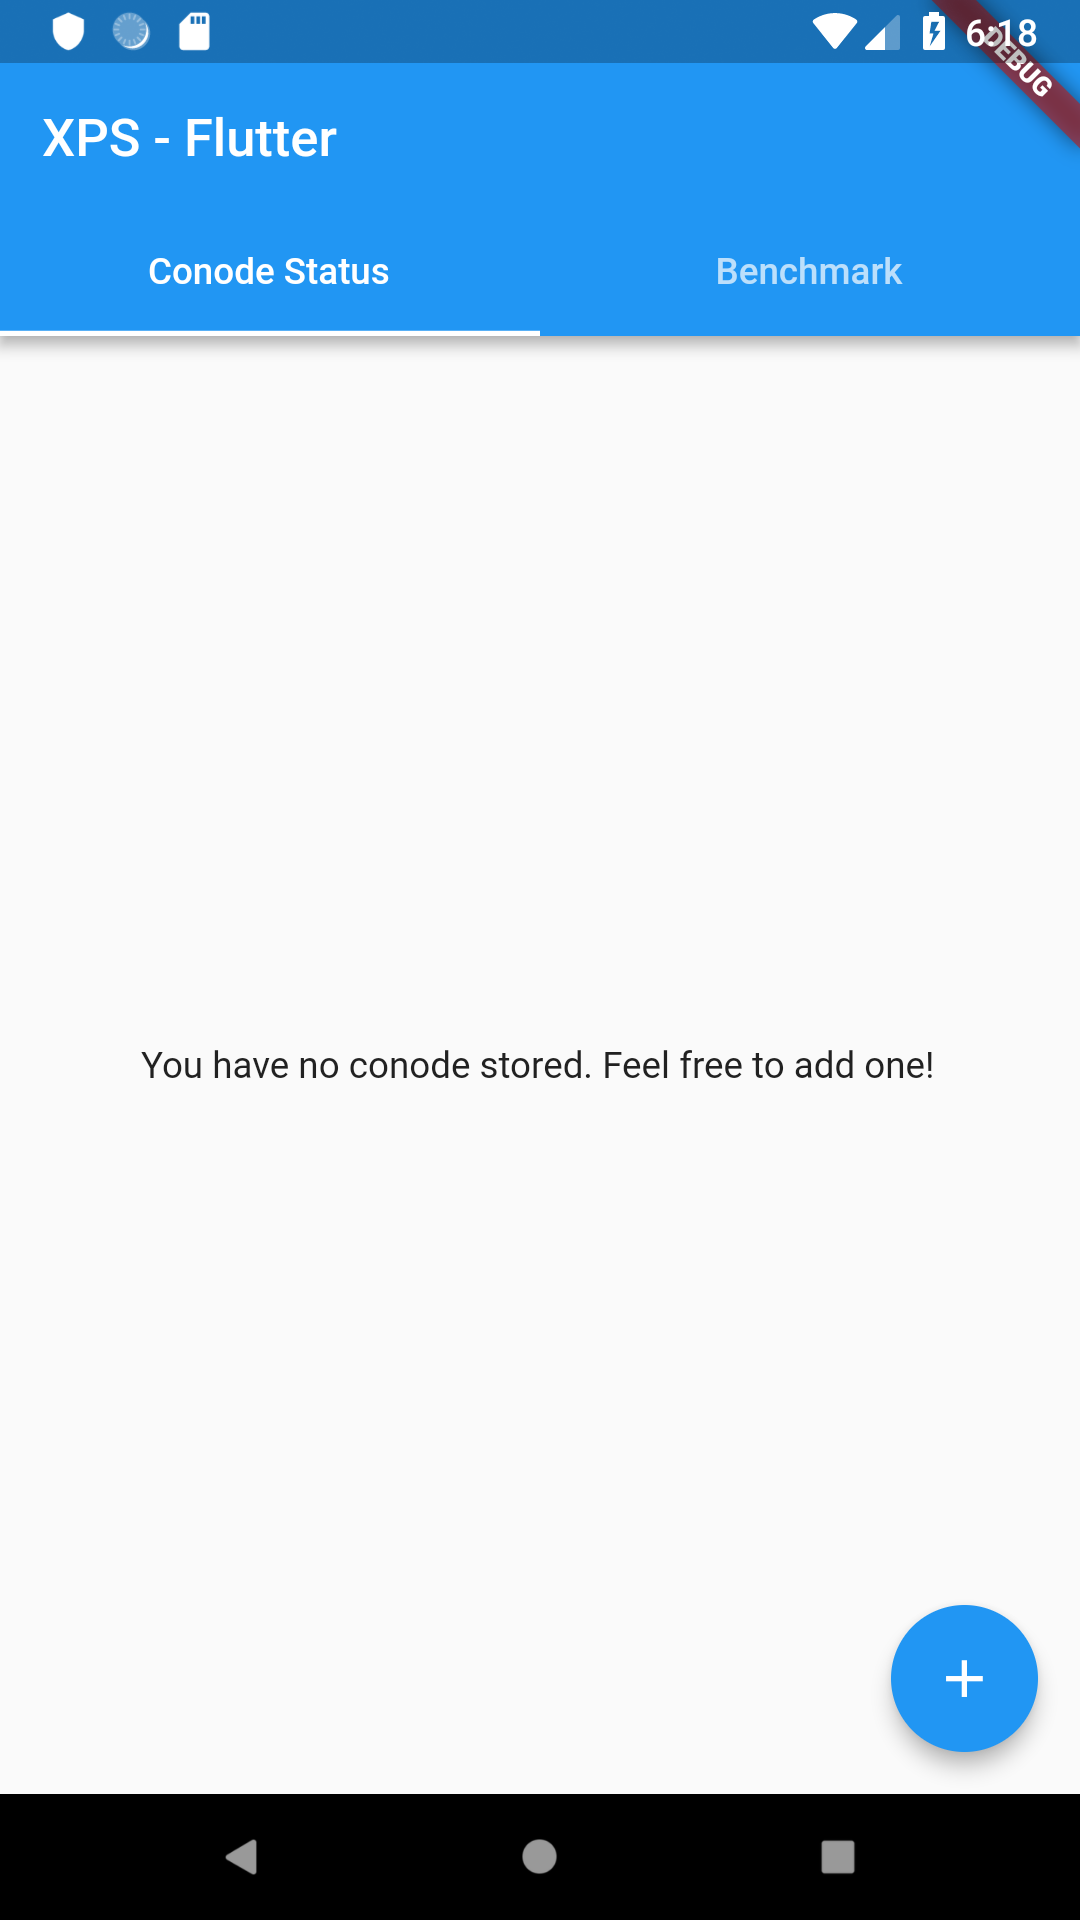
\includegraphics[width=0.35\textwidth]{img/Flutter_layout_android.png}
	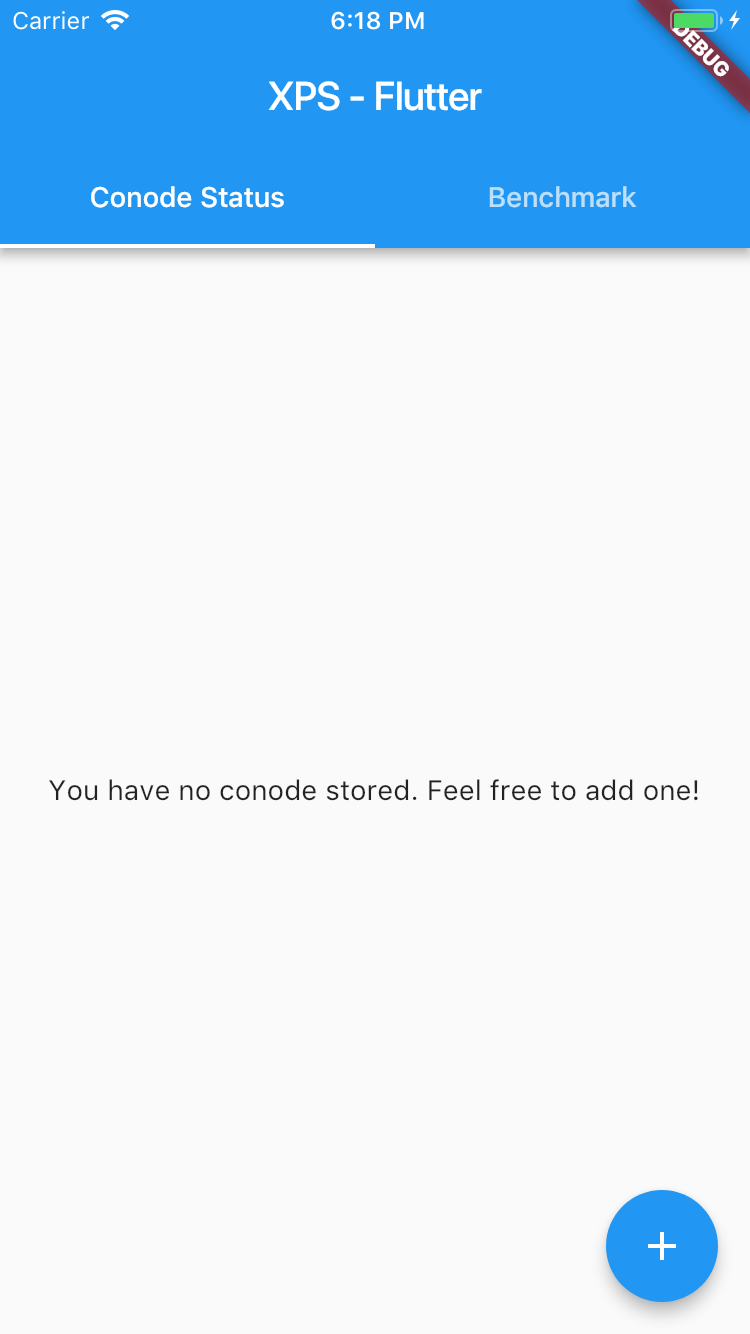
\includegraphics[width=0.35\textwidth]{img/Flutter_layout_ios.png}
	
	\caption{Flutter: Material Design Tab layout in Android (left) and iOS (right)}
	\label{fig:flutter_material_design}
\end{figure}

Flutter is a free and open-source cross-platform framework developed by Google. It allows building mobile applications for iOS and Android sharing the same Dart codebase.\\

Before detailing the work done with this framework, here are the important parts:

\begin{itemize}
	\item All features work on Android but not on iOS (see subsection \ref{sub:flutter_ease_integration}).
	\item Distributed under BSD 3-Clause, allows using Flutter for open source purpose and/or commercially.
	\item Integration requires either to have Swift and Java bindings or a full Dart rewrite
	\item Debugging is fully featured and stable.
	\item Provides UI widgets and layouts necessary, but those are not "aware" of the platform they're displayed on.
	\item Easy deployment on both platforms.
	\item Cryptographic operations much slower on Android, unknown on iOS.
\end{itemize}


\subsection{Implementation}
The implementation was done using the Flutter plugin flutter\_barcode\_reader\footnote{\url{https://github.com/apptreesoftware/flutter_barcode_reader}}. It works perfectly on both iOS and Android.

On the Android platform, it is possible to get a conode's status as the cothority was also ported to a Java version, with websockets working.\\
There is no working implementation of the websocket communication with a conode for iOS. The reason of this are later detailed in subsection \ref{sub:flutter_ease_integration}.

Flutter provides a SharedPreferences mechanism natively which allows the developer to save information on the device. Using it, the current application can store JSON information about a conode to permanent memory and retrieve it when starting. This storing mechanism works on both mobile platforms.

The 100 Schnorr signatures with validation were implemented for Android but not for iOS. The reason is also discussed in subsection \ref{sub:flutter_ease_integration}.

\subsection{Licensing}
Flutter is distributed under the BSD 3-clause  license\footnote{\url{https://opensource.google.com/projects/flutter}}, which allows usage, modification, distribution, commercial use, as long as the project includes the copyright and the license. It also forbids usage of Google and its associated products' trademarks and any liability charge.

\subsection{Ease of integration}
\label{sub:flutter_ease_integration}
Flutter relies on the Dart language. As there was no Dart version of the cothority, the integration here was trickier than for other JavaScript based frameworks. For Android, the Java version of the cothority was used with success, but for iOS there was no convenient way to get the cothority working. This is further discussed in appendix \ref{sub:appendix_flutter_integration}.

\subsection{Debugging}
After installing the Flutter (official) plugin in Android Studio, debugging in Flutter is fully functional and provides all expected features: breakpoints, state exploration, step by step debugging... It is integrated with Android Studio's UI.

\subsection{UI widgets and layouts}
Flutter provides a complete UI library, and lets the developer choose between a Material Design (Android) style or Cupertino (iOS) style. Widgets and layouts are not platform aware. A solution to this is detailed in appendix \ref{sub:appendix_flutter_ui}.

\subsection{Deployment}
Deploying a Flutter app is a similar experience to deploying a native Android application, be it for Android or iOS devices. Either by using as single command line or using Android Studio's run button, the application is packaged, installed and run directly on the chosen device. Same goes for debugging. It's important to notice that this is the only framework for which there was no recurring build issues.\\ 
Flutter also provides a Hot Reload feature, which works well in combination with the debugger.\\

Both Unit and UI testing frameworks for Flutter are provided to the developer by default\footnote{\url{https://flutter.io/docs/testing}}, allowing testing classes and widgets. Flutter also provides integration testing, which is important for recurrent use cases. The testing framework is notably well documented.

\subsection{Benchmark}
As mentioned in subsection \ref{sub:flutter_ease_integration}, the iOS version of the app cannot perform Schnorr's signatures and run benchmarks at the time of writing of this report.

On Android, the 100 Schnorr signatures and validations were completed in 70795ms. This is way slower than NativeScript on Android, which seems to be related to garbage collection occurring more often with the Java implementation. Also, the implementation for this application is single threaded (as in JavaScript) but the UI is still responsive, meaning that the main thread still completes UI operations before resuming the benchmark, hence allocating CPU time for the UI refresh and adding some time to the final benchmark result.

\newpage
\section{Go Mobile}
Go Mobile is an experimental project developed by the Go Team and Google that provides tools to use Go on mobile platforms.\\
After some research about the advancement of the project, some dead-ends were encountered and put a halt on further investigation. Here is a quick overview of what's important to know about this framework:


\begin{itemize}
	\item No UI library! Currently, the only way to have a UI is by writing a UI library in Go using the OpenGL accessible calls. As the development of a UI library was far beyond the scope of this project, the application development was dropped.
	\item Access to camera and storage not possible via Go code.
	\item Very little documentation, even on examples.
	\item Distributed under BSD 3-Clause, allows using Go Mobile for open source purpose and/or commercially.
\end{itemize}



\subsection{Implementation}
As previously mentioned, the lack of a UI library put a halt on the development of the application. There also was no way to access the camera or internal storage using the Go framework. 

\subsection{Licensing}
Go Mobile is distributed under the BSD 3-clause  license\footnote{\url{https://github.com/golang/mobile/blob/master/LICENSE}}, which allows usage, modification, distribution, commercial use, as long as the project includes the copyright and the license. It also forbids usage of Google and its associated products' trademarks and any liability charge.

\subsection{Ease of integration}
This is unknown for the same reason given before. Even though, the process of integration would require a deep adaptation of the Go code, e.g. external types are currently not supported\footnote{\url{https://github.com/golang/go/issues/12570}}.

\subsection{Debugging}
Not tested. However, from the Go repository we can see that debugging still is experimental, as for example stack traces are incorrect in some cases\footnote{\url{https://github.com/golang/go/issues/22716}}.

\subsection{UI widgets and layouts}
No UI library! Currently, the only way to have a UI is by writing a UI library in Go using the OpenGL accessible calls. There exists some attempts to write a UI library or create bindings to Qt, but they are experimental or unmaintained.

This is the main reason why no application was developed using Go Mobile, as the development of a UI library was far beyond the scope of this project.

\newpage
\section{Xamarin}
Xamarin is a cross-platform framework maintained by Microsoft that allows creating applications on Android, iOS and Windows platforms using a single .NET codebase (using C\# language).\\
The development of the application using Xamarin was also halted at its very beginning. Here is a list of reasons why development was halted on this platform, and other important points:

\begin{itemize}
	\item The integration process has the same limitations as for Flutter (see subsection \ref{sub:xamarin_integration}).
	\item Integration requires either to have Swift and Java bindings or a full .NET rewrite.
	\item Given the previous points, it was decided to spend the time allocated on Xamarin to work on Ionic, another framework not featured on the to-do list of this project.
	\item Xamarin is distributed under the MIT License, which allows using Xamarin for open source purpose and/or commercially.
\end{itemize}

There is therefore no subsection for Debugging, UI, Deployment and Benchmarking for Xamarin.

\subsection{Implementation}
No feature was implemented, because of the foreseen too long time for integration (see \ref{sub:xamarin_integration}).

\subsection{Licensing}
Xamarin is distributed under the MIT license\footnote{\url{https://github.com/xamarin/Xamarin.Forms/blob/master/LICENSE}}, which allows usage, modifications, distribution, commercial use, sublicensing.\\

\subsection{Ease of integration}
\label{sub:xamarin_integration}
The integration process was found to be similar to Flutter (subsection \ref{sub:flutter_ease_integration}). There was only two options: either rewrite the cothority library in .NET or rewrite it in Swift for the iOS application and use the existing Java library for the Android application, by creating bindings to the .NET code. 
This redundancy made Xamarin look uninteresting for the purpose of this project, as it would still require a full rewrite of the library in one particular language. 

\newpage
\section{Ionic}

\begin{figure}[!htb]
	\centering
	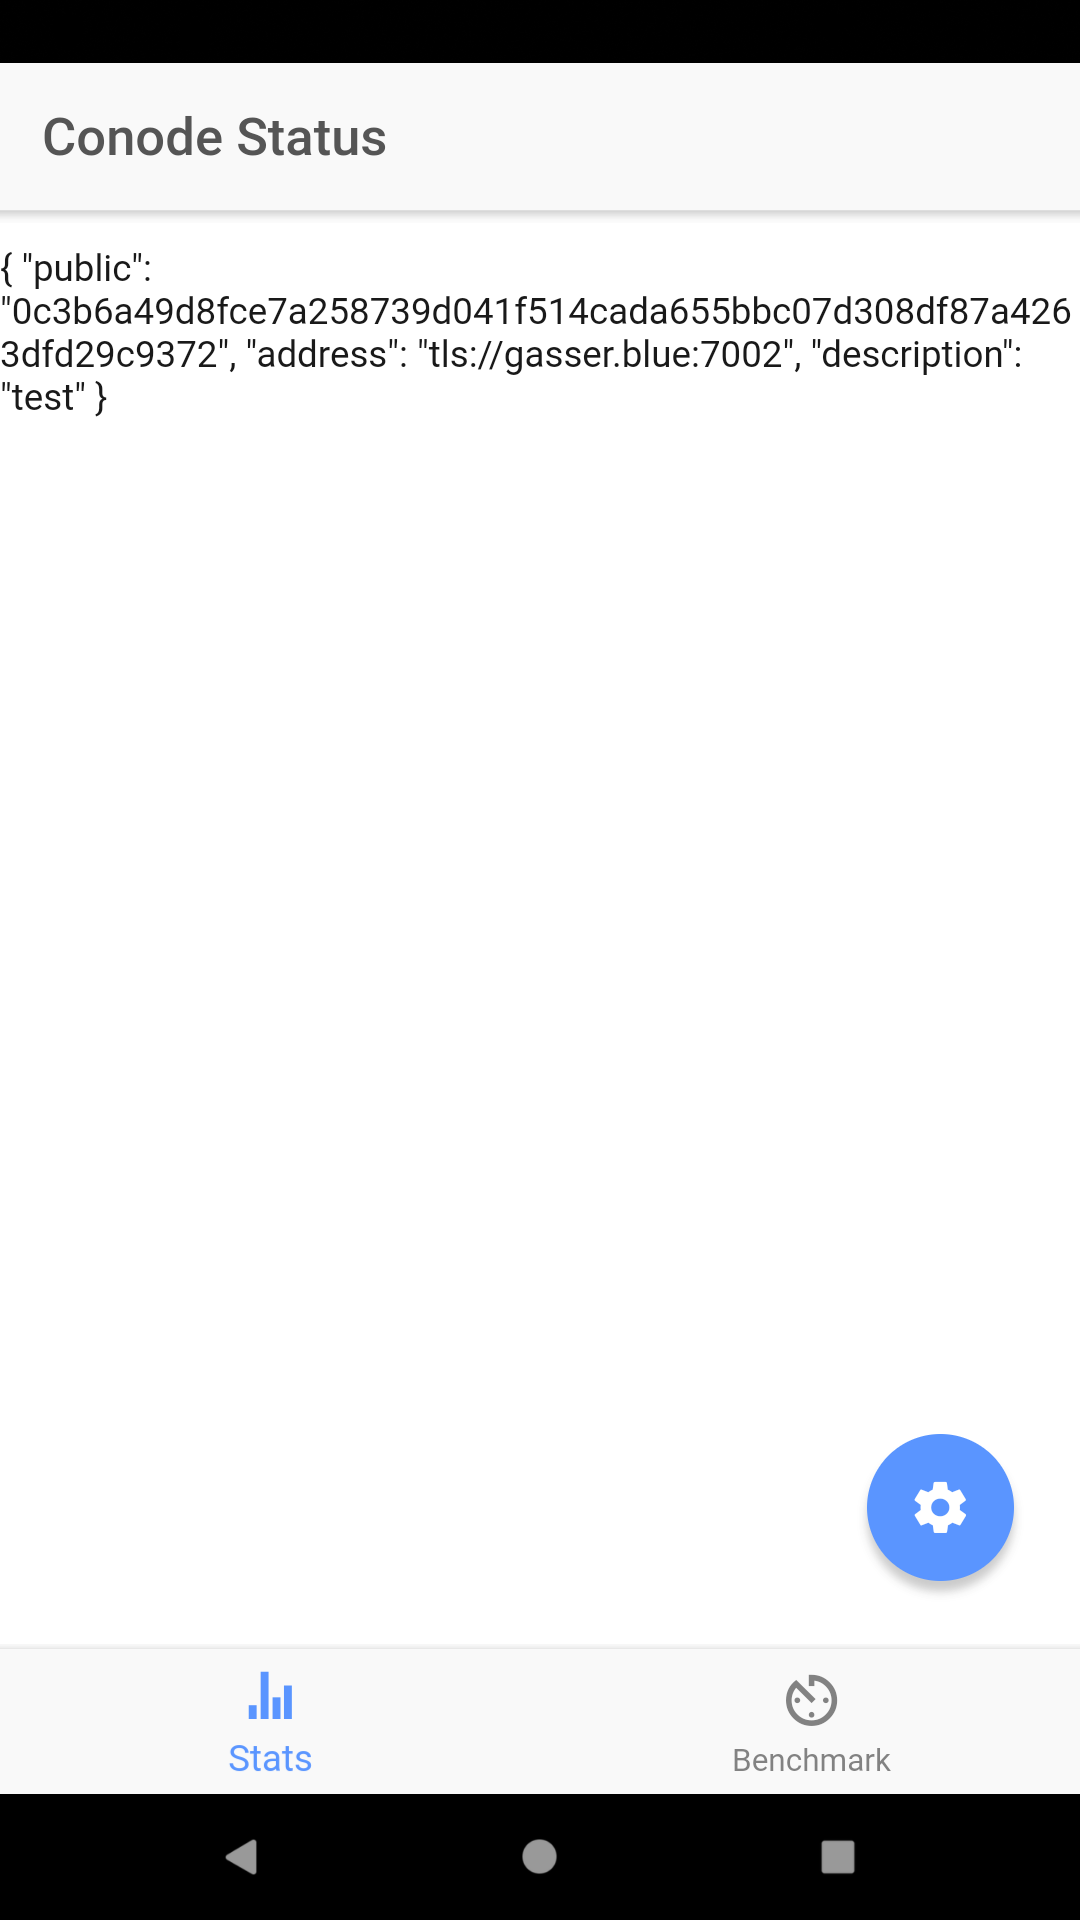
\includegraphics[width=0.35\textwidth]{img/ionic_layout_android.png}
	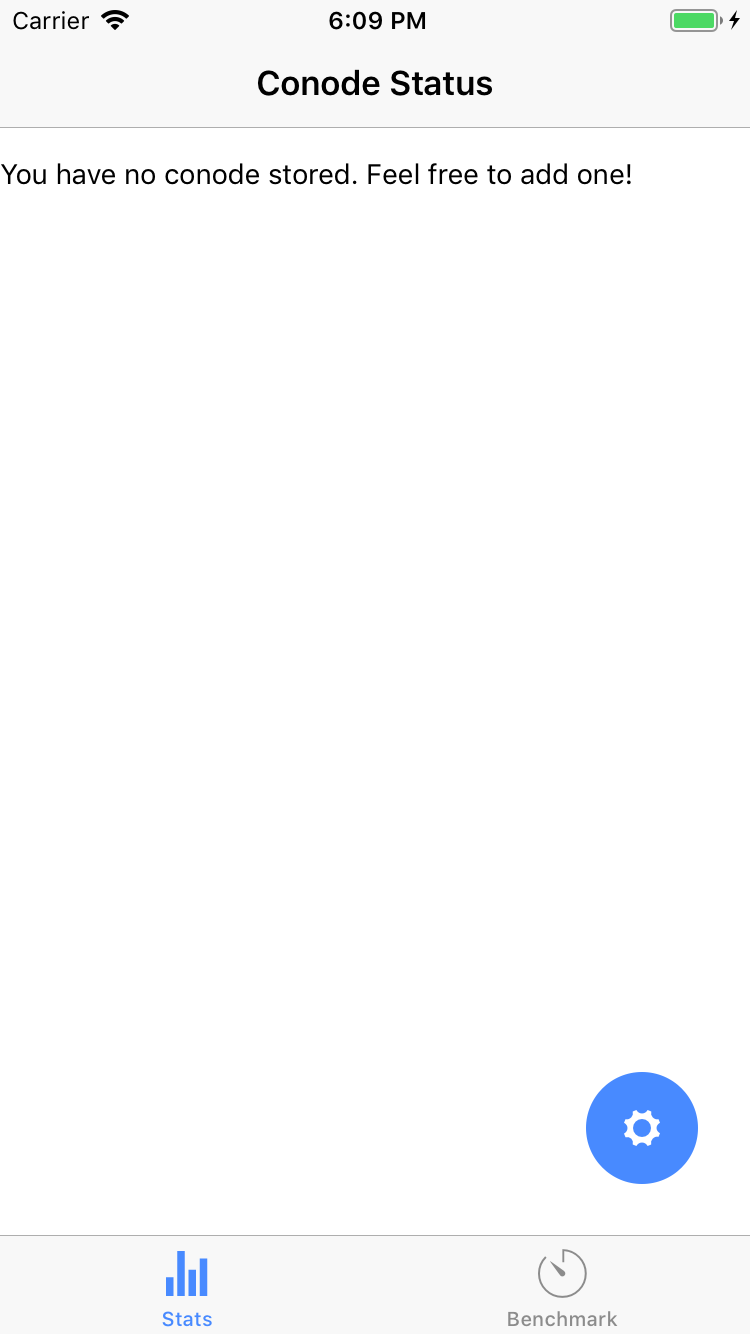
\includegraphics[width=0.35\textwidth]{img/ionic_layout_ios.png}
	
	\caption{Ionic: Tab layout in Android (left) and iOS (right)}
	\label{fig:ionic_layout_comparison}
\end{figure}

Ionic is a cross-platform framework developed by Drifty, that relies on HTML5, CSS and TypeScript/JavaScript to produce cross-platform mobile applications. As for some other frameworks, the fact that it relies on JavaScript simplifies the integration process.\\

Here are some important points about this framework:

\begin{itemize}
	\item Websockets do not work in the current implementation on both Android and iOS, but Schnorr signatures do.
	\item Distributed under the MIT License, allows using Ionic for open source purpose and/or commercially.
	\item TypeScript/JavaScript code, simplifies the integration of existing JavaScript libraries.
	\item Debugging is done with Chrome DevTools, less convenient than integrated solutions within IDEs like WebStorm, but still stable and fully featured.
	\item No integrated test framework.
	\item Provides UI widgets and layouts necessary.
	\item Deployment easy on both platforms once few build issues are addressed.
	\item Schnorr signing runs at correct speed on Android,  fast on iOS.
\end{itemize}

Let's now talk about the implementation of the features.

\subsection{Implementation}
The QR Code reader was implemented using the Ionic's qr-scanner\footnote{\url{https://ionicframework.com/docs/native/qr-scanner/}} module. It works on both Android and iOS.


Websocket support is not documented and as such not working on this platform. Some third party modules were tested but did not work, as they were developed years ago for older Ionic versions and olders mobile OSs.

Ionic natively provides a storage mechanism which was used for the application and is flawlessly working on both platforms.

Schnorr's signatures runs on both platforms without much adaptation needed. Again, it freezes the UI thread.

\subsection{Licensing}
Ionic is distributed under the MIT license\footnote{\url{https://github.com/ionic-team/ionic/blob/master/LICENSE}}, which allows usage, modification, distribution, commercial use, sub-licensing.\\

\subsection{Ease of integration}
Contrary to NativeScript, Ionic did not require readapting JavaScript code to use specific modules for Ionic. Hence, the integration was quite fast, although websockets don't work. Currently the app only displays the decoded JSON string from the QR Code reader.

\subsection{Debugging}
Debugging is done using Chrome DevTools. Although it does not lack of primordial features like breakpoints and stack exploration, its usage is not convenient for the developer, as detailed in appendix \ref{sub:appendix_ionic_debugging}.

\subsection{UI widgets and layouts}
Ionic provides a well featured UI library. It includes by default a Tab layout, and other platform specific widgets like floating action buttons.\\
The look and feel of Ionic apps is a mix of Cupertino style (iOS) and Material Design (Android), as seen in fig. \ref{fig:ionic_layout_comparison}.

\subsection{Deployment}
The build process for Ionic applications is stable once some well known issues are fixed by using specific command flags (see appendix \ref{sub:appendix_ionic_deployment}).\\

Ionic does not provide a test frameworks, but can be configured to work with Karma and Jasmine for unit testing and Appium for UI testing.\\

A more detailed discussion is given in appendix \ref{sub:appendix_ionic_deployment}.

\subsection{Benchmark}
Benchmarks were run on both platforms, with promising results.\\

On Android, the benchmark completed in 17313ms which is slower than on NativeScript but can still be considered as acceptable.\\

On iOS, the benchmark completed in 3822ms, which is a little bit faster than NativeScript on Android, by a negligible margin. Further investigation were conducted, and showed that the multiplication between a point and a scalar when generating or verifying a Schnorr signature is 1.1x faster than compared NativeScript Android, and hash computation is roughly 3x faster!\\
Ionic is therefore the framework with the best compromise of speed between the iOS and Android platforms.

\newpage
\section{Summary}
Appendix \ref{sec:summary_table} summarizes in the form of a table the evaluations on all tested frameworks. Some criteria are evaluated by their ease of usage, which is a subjective assessment based on the (trying-to-be) objective discussion on frameworks in previous sections. For some framework, there is an unknown value for the evaluation: it's recommended to read the corresponding framework section to understand why it is marked as such.\\

From the discussion on frameworks we can say that there now exists lots of cross-platform frameworks using different languages, but JavaScript keeps a stronger presence. For other frameworks, there is often a need to rewrite the cothority in a platform's native language, thus mitigating the advantage of a cross-platform framework. On the licensing theme, the vast majority of those frameworks are now open-source, as it is now viewed as mandatory by developers.\\

The results displayed in appendix \ref{sec:summary_table} give a general idea of the work necessary in order to migrate to other frameworks than NativeScript, along with the advantages and trade-offs to do so. 

We can quickly see that one particular framework can be quickly discarded: Go Mobile is too experimental and does not provide a functional UI library. Others require a total rewrite of the codebase and seem thus less interesting; this is the case for Flutter and Xamarin, for which it is necessary to question the advantage of rewriting code for a cross-platform framework rather than target directly native environments.

Often websocket communication does not work out of the box and needs some extra research. This isn't surprising as it was necessary to patch the NativeScript websocket in order to get it working.

Also, building iOS applications has often been an issue as Apple released their Xcode 10 recently, completely upgrading the build engine. Surely those issues will be addressed in the near future, but this has handicapped the comparison on the iOS platform for this project.

UI libraries are usually well featured, but sometimes might need third party packages to be truly complete. Depending on the wanted style, one may prefer Ionic approach of a single design for all platforms, or NativeScript's platform-aware widgets and layouts.

Finally, in terms of performance, Ionic truly stands out compared to others, and React Native has similar performances on Android, but we cannot know for now on iOS. Usually, the gap in performance is due to the implementation of the multiplication used for the Schnorr signature and its validation.\\

This concludes the evaluation of those 6 different cross-platform frameworks. As we can see, there is no framework clearly standing out compared to others. NativeScript might still be the easiest choice in term of integration and deployment, but this is due to the work already put in adapting the cothority JavaScript codebase to this framework. Unfortunately, the extreme slowness of the multiplication for the Schnorr signature on iOS severely mitigates the possibility of keeping this framework.
Ionic presents interesting integration ease and great performances, but can still be improved in terms of debugging, testing and deployment. React Native is too unstable in deployment and debugging to be recommended.
 Flutter and Xamarin both present the drawback of requiring a codebase rewrite, and Go Mobile does not provide any UI library.\\
 
 The perfect cross-platform framework for the wanted use case might not exist yet, but fortunately there are some promising ones.

\newpage
\appendix
\section{Comparing evaluated frameworks}
\label{sec:summary_table}
\hspace{-1cm}
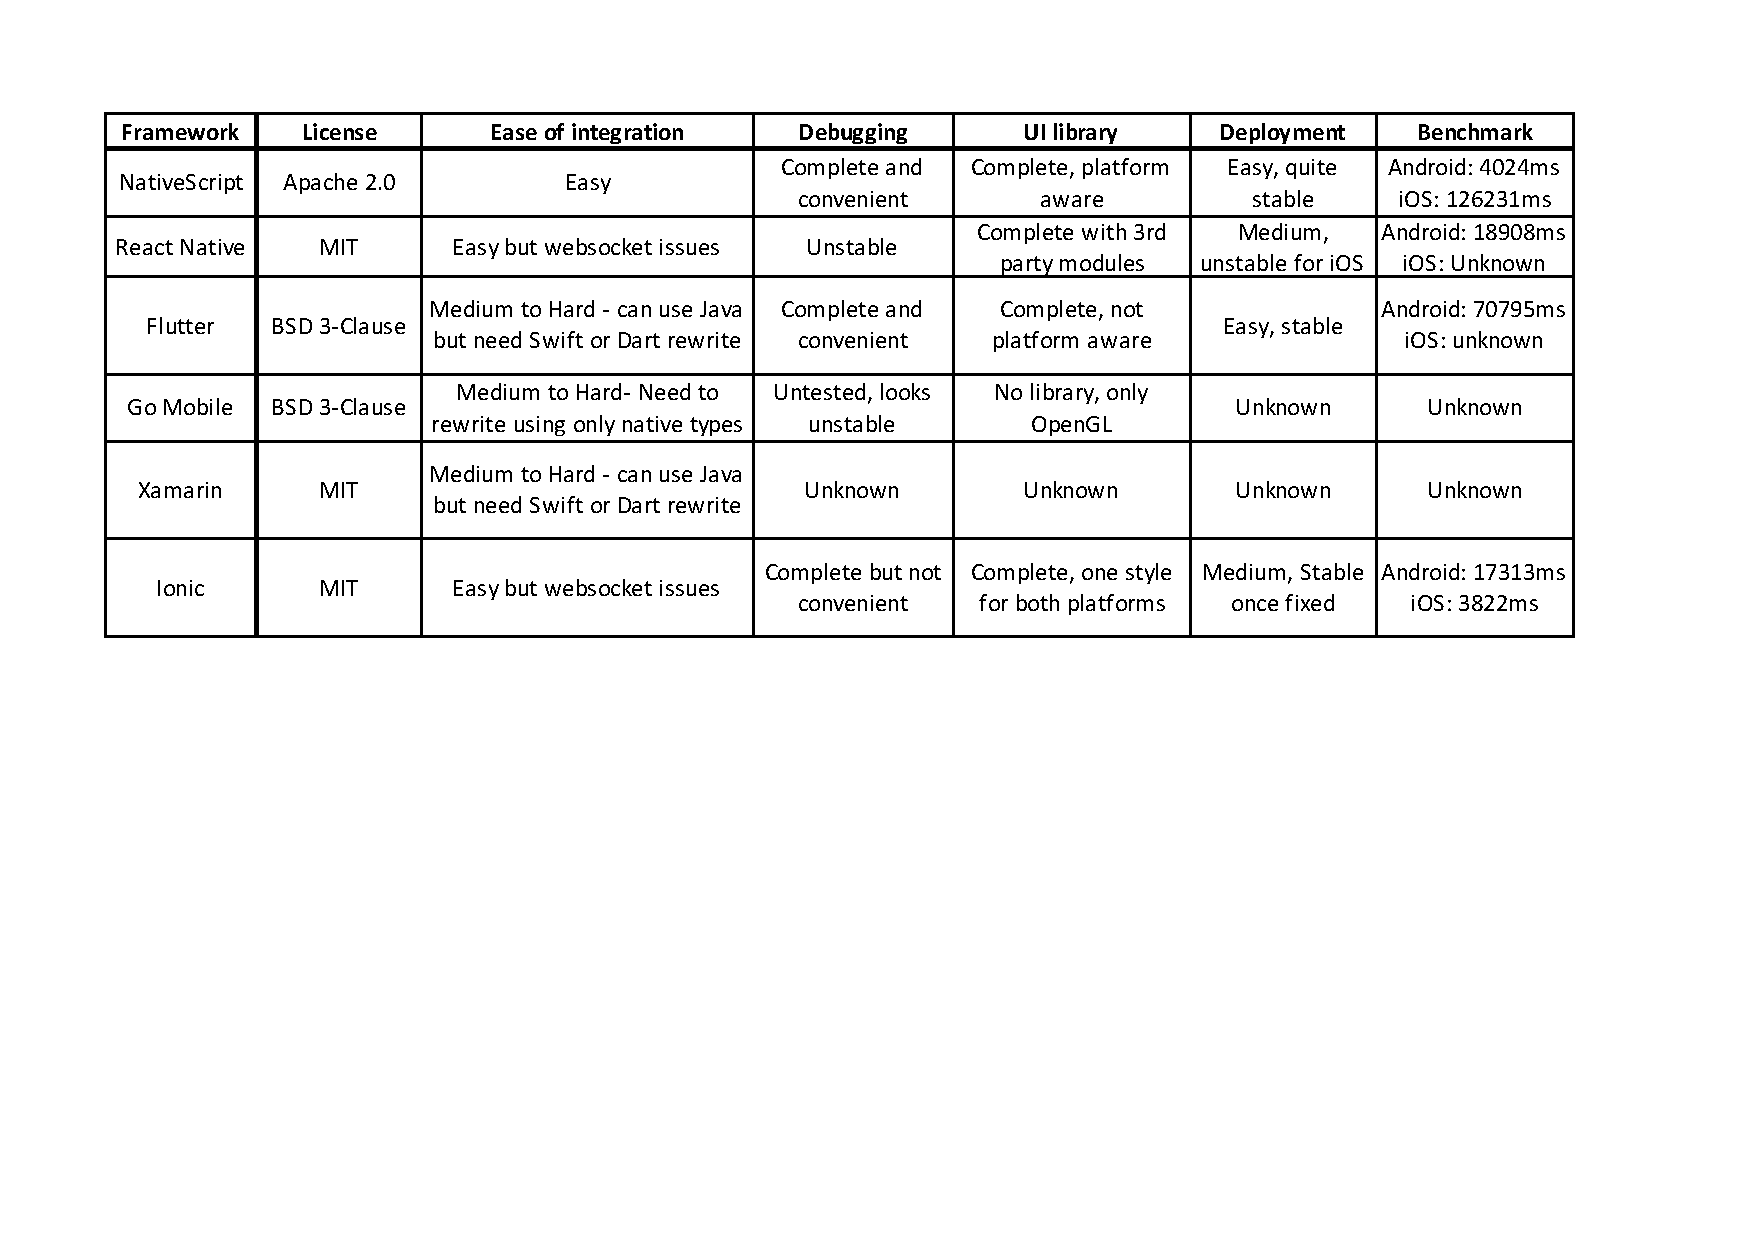
\includegraphics[scale=0.6]{frameworkComparison.pdf}

\section{In details: NativeScript}
\subsection{Deployment}
\label{sub:appendix_nativescript_deployment}
Similar to the popcoin app, the deployment of the application is not a one click operation. It is first necessary to install the required Node.js packages in order to build the app. However, in order to get websockets running on Android and also fix a crash at the app's start, some patches must be applied after downloading the Node.js packages and before running the app. In order to get things done in the correct order, as it was done for popcoins, an included Makefile does all this for the developer. \\
Then, using the tns CLI, the developer can deploy the app in either run or debug modes, on both mobile platforms. On iOS, it might be necessary in some cases to uninstall the application before installing it, which results in data loss for this app but fixes the installation issue. Also, with recent updates, it is necessary to downgrade the build system for the workspace if the user has Xcode 10 installed. \\
All those procedures are described in a README.MD file, located in the NativeScript subfolder of this project.\\

NativeScript supports unit testing with JavaScript test frameworks such as Mocha\footnote{\url{https://mochajs.org/}} or Jasmine\footnote{\url{https://jasmine.github.io/}}. Running unit tests on an emulator or a physical device is done by a single line command, although the packages and patches should first be applied by using the Makefile as discussed previously.\\
By adding the official package nativescript-dev-appium\footnote{\url{https://github.com/NativeScript/nativescript-dev-appium/}}, one can then write UI tests for the NativeScript application. It allows interacting with all UI components, and provides a high flexibility through configuration files determining the specific device to run the tests on.


\section{In details: React Native}
\subsection{Debugging issues}
\label{sub:appendix_react_debugging}

Debugging on React Native can still be improved as the process is unreliable in some cases.\\

\begin{figure}
	\centering
	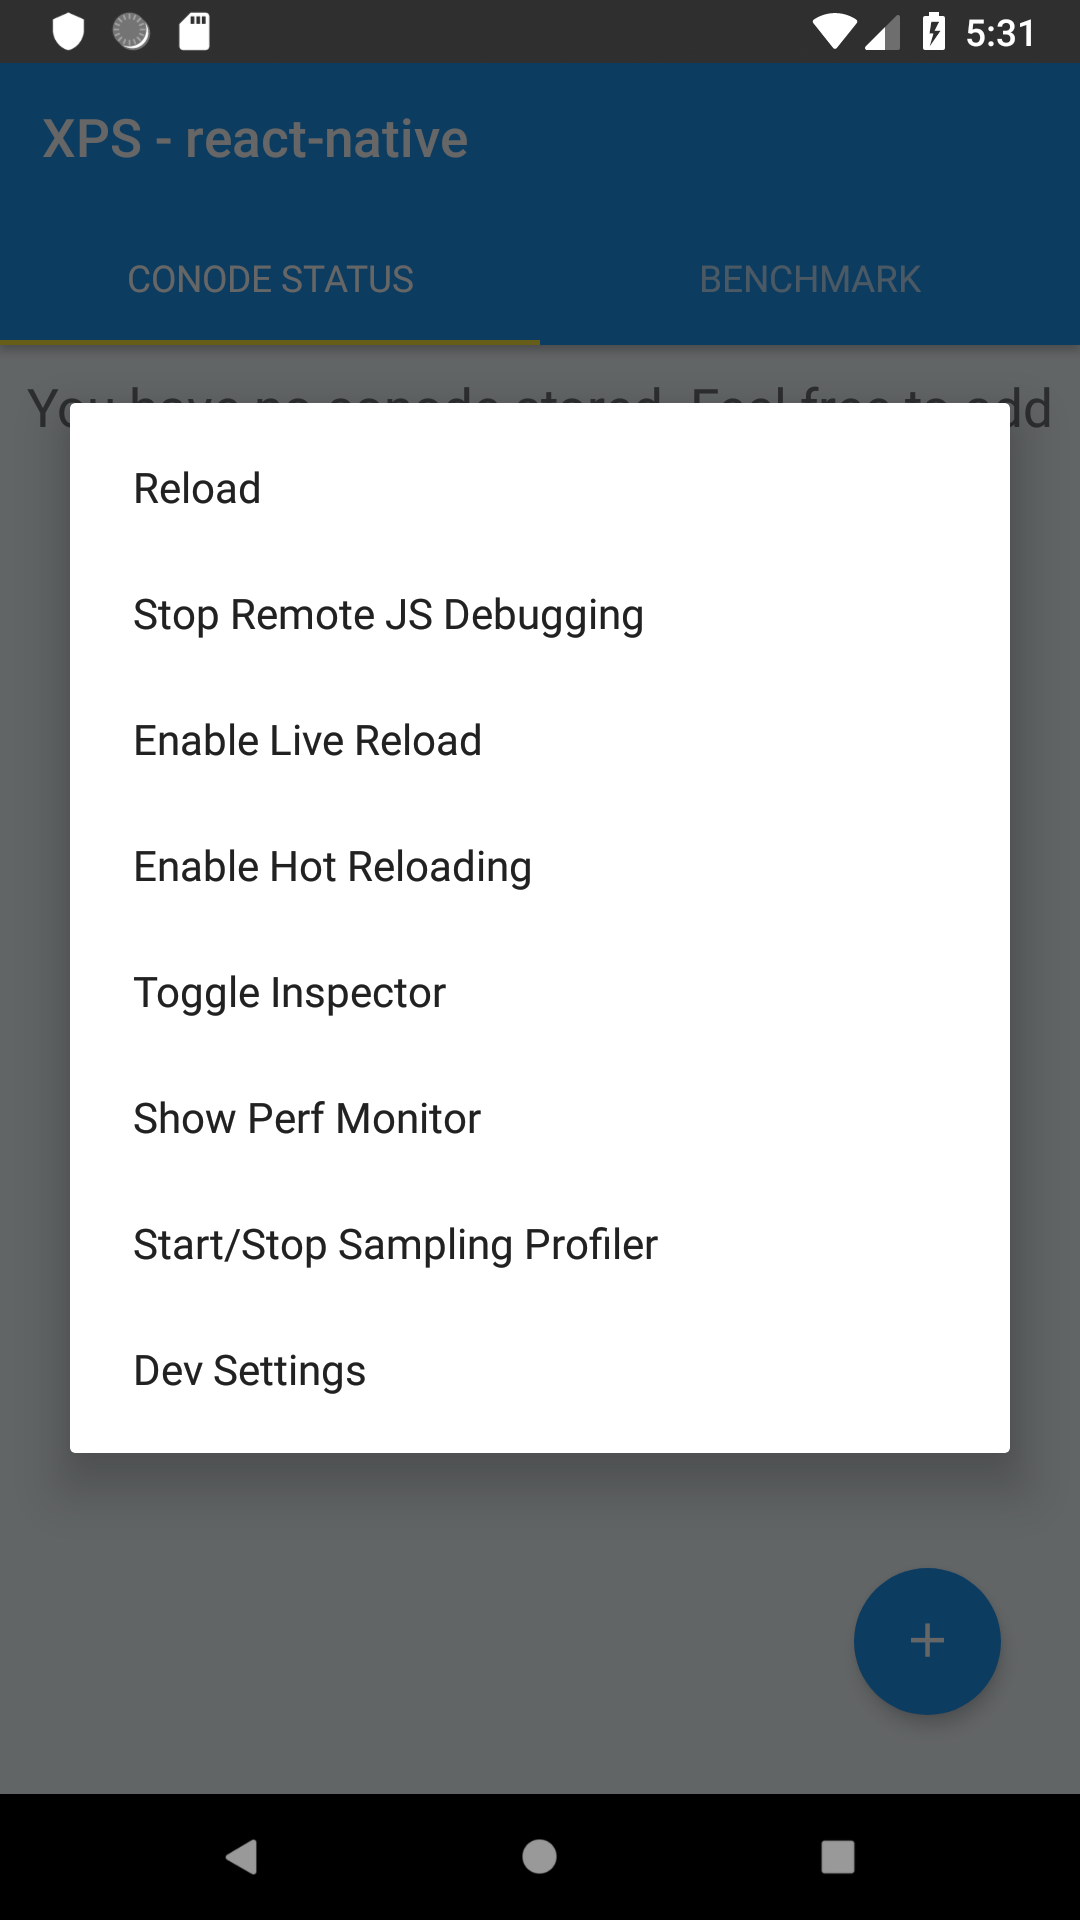
\includegraphics[width=0.35\textwidth]{img/react_dev_menu.png}
	
	\caption{React Native: Internal menu to enable Hot Reloading and remote debugging}
	\label{fig:react_dev_menu}
\end{figure}

It is possible to debug applications directly into IDEs like WebStorm. This allows the developer to set breakpoints and explore the state of variables and memory at a given time, like it is the case for many frameworks. This feature (called Remote JS Debugging) can be enabled through an internal menu of the app like shown in fig. \ref{fig:react_dev_menu}.
However, two main issues can arise and cause the usage of React Native's debugger to be way more difficult.\\

First, the application will sometimes fail to connect to the remote debugger. The best solution to fix this issue is to kill the Metro Bundler (which opens in a new terminal window) with ctrl+c, uninstall the app on emulators and re-run the app. This process removes data generated from the application, and can waste some precious development time.\\

The second issue arises more often and is quite problematic. As for many frameworks, React Native provides a "Hot Reloading" feature, also to be enabled by using the internal menu shown in fig. \ref{fig:react_dev_menu}. With it, when a developer updates a JavaScript file of the application, the development server will only reload the updated JavaScript file on the application running, hence updating the app (few seconds) amazingly fast without the need to rebuild the entire application (which can take minutes). This feature is great to reduce the time waiting for the build process to finish. 
In the case of React Native, this feature cannot be used with debugging as it leads to a line-shift in breakpoints. \\
Here is an example: let's say a developer sets a breakpoint at line 25 of a JavaScript file. Then the developer adds 2 lines of code before line 25 to the same file, with Hot Reloading enabled. In the IDE, the breakpoint now lies at line 27. The Hot Reloading feature ensures the file is uploaded to the application, which is refreshed with the modifications done to the file. But here, the application will halt when it encounters the instruction at line 25, not 27! And setting a new breakpoint after the Hot Reloading will still result of a shift of 2 lines between the wanted breakpoint and the line where the application will halt. The solution here is to disable Hot Reloading and rebuild the app, and not use Hot Reloading at all while debugging. This feature could have been useful but is unfortunately unreliable.

\subsection{Deployment}
\label{sub:appendix_react_deployment}
With the React Native framework, a development server is created when the application is run. This local server packages a base app and install it on the wanted devices. Then, any changes done to JavaScript files are passed to the development server which will send them to the running application. When the developer wants to release an application to a production environment, the source files and the runtime used to execute JavaScript files are packaged into a .apk file to be installed on devices.\\
The implementation of this deployment architecture has some issues, as discussed in subsection \ref{sub:react_debug}. \\
Unfortunately on iOS an update of the React Native framework combined with the new Xcode 10 leads to builds crashing. Falling back to an older version of the framework and the legacy build system of Xcode did not fix the issue. It can still be mentioned that the deployment on Android seems experimental but works most of the time when not using Hot Reloading and Debugging together.\\

Unit testing in React Native is done by using Jest\footnote{\url{https://jestjs.io/en/}}, React's own test framework. It does not provide UI testing but has an interesting feature called snapshots. Snapshots allow detecting potential unwanted changes in the UI generation between two tests by saving snapshots of the generated UI to a local file. This does not replace a UI test framework, but it possible to integrate Appium tests to Jest tests\footnote{\url{https://medium.com/@7ynk3r/react-native-e2e-testing-with-appium-on-sauce-labs-8920195b8a54}}. The manipulation is quite hacky but provides further testing for the application.

\section{In details: Flutter}
\subsection{Ease of integration}
\label{sub:appendix_flutter_integration}
There were two choices to get the cothority library working on Flutter. The first one was to rewrite the whole codebase in Dart, but this choice was not followed as it was judged more interesting to spend time testing other frameworks rather than writing code from scratch. \\

\begin{figure}
	\centering
	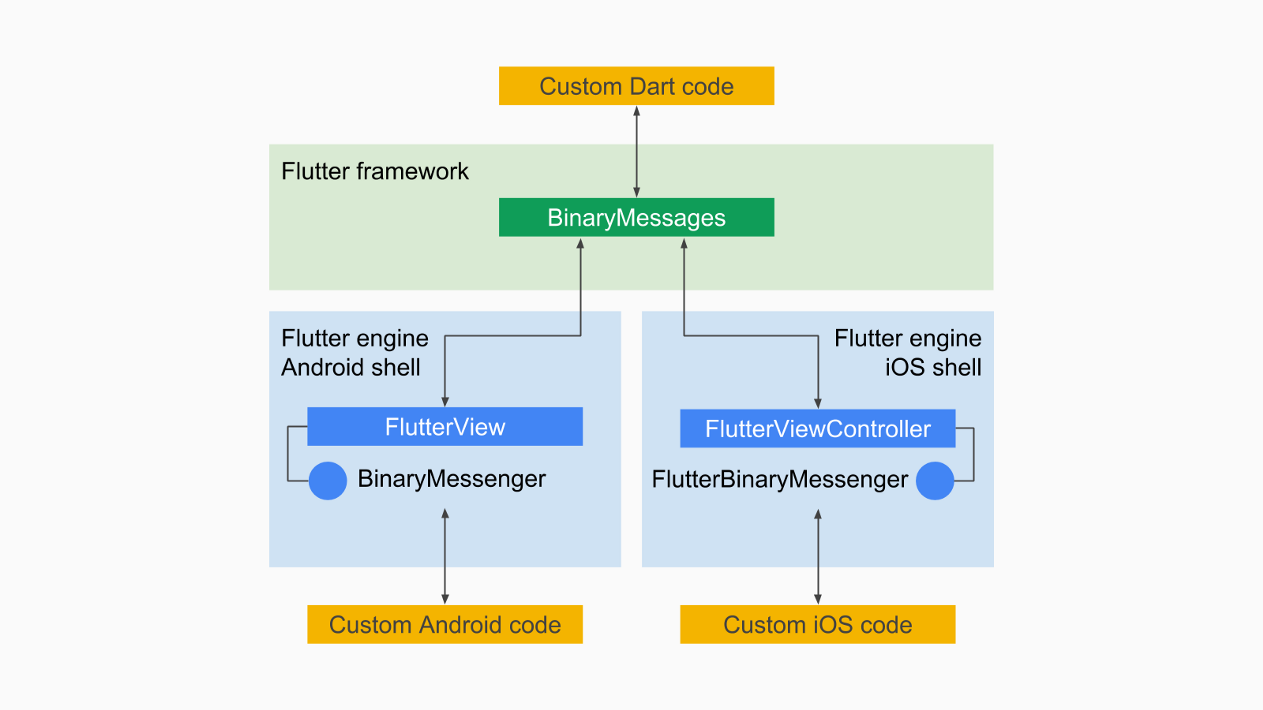
\includegraphics[width=0.85\textwidth]{img/Flutter_native_code.png}
	
	\caption{Flutter: Running platform specific code, \copyright \href{https://medium.com/flutter-io/flutter-platform-channels-ce7f540a104e}{Mikkel Ravn}}
	\label{fig:flutter_native_code}
\end{figure}
The second option was to write only the application logic in Dart, but have it call routines programmed in native languages (Java for Android, Swift for iOS). Those routines would be responsible for the library related work, such as the Schnorr's signature/validation and websocket communication. Fig. \ref{fig:flutter_native_code} gives an idea of the architecture of the code.
This was the path followed, and the following subsections describe the work done for both Android and iOS.

For Android, the integration was facilitated by the already existing Java version of the cothority. A Java class was written to create the bridge between the Dart calls and the Java library, hence exposing communication with conodes via websockets and Schnorr operations to the Dart code part of the application.\\
This integration works flawlessly: websockets and Schnorr signatures work as intended.

For iOS, there was no Swift version of the cothority available. An attempt was made to create a binding from the original Go library to a iOS oriented Swift code, by using the "gomobile bind" feature to create an iOS framework. This failed as this binding operation only supports a limited set of types, which the Go version of cothority does not use exclusively.\\
An other attempt was to follow the work done for the prifi mobile application\footnote{\url{https://github.com/dedis/prifi/tree/ios-project}} to get the Go cothority libraries working on iOS. In order to use the background service responsible for communications on iOS, the developers of prifi mobile have had the application request the creation of a VPN. Unfortunately, VPNs on iOS do not work\footnote{\url{https://github.com/flutter/flutter/issues/21666}} with Flutter and in general there is no support for proxies\footnote{\url{https://github.com/flutter/flutter/issues/20704}}. Thus, there was no possibility to readapt the code from the prifi mobile application for this application.\\
As such there remains two possibilities to get the features wanted working on iOS: either rewrite the libraries in Swift/Objective C (with existing libraries providing support for ed25519) or rewrite them in Dart (no known ed25519 library at the time of the project). It was consequently decided to not spend more time trying to adapt the code on iOS, but explore frameworks instead.

\subsection{UI library}
\label{sub:appendix_flutter_ui}
Flutter provides a complete UI library, and lets the developer to choose between a Material Design (Android) style or Cupertino (iOS) style. Although the UI library offers more widgets and layouts than other cross-platform frameworks, the code written to describe the UI of an application is not exactly cross-platform. When in NativeScript a tab layout would automatically have an Android look and feel on Android and an iOS look and feel on iOS, here in Flutter the developer has to specify manually the look and feel of the whole application and use widgets/layouts corresponding to it. For this project, the Material Design style was chosen for the application. The application thus look exactly the same on iOS and Android, as shown in fig. \ref{fig:flutter_material_design}.\\
In order to share the same codebase but have a native look and feel on each platform, an option is to write a Factory\footnote{\url{https://medium.com/flutter-io/do-flutter-apps-dream-of-platform-aware-widgets-7d7ed7b4624d}} class to use throughout the application's code when creating UI. It's easy to understand why this architecture was chosen by the Flutter team, as not every widget on one platform has its counterpart on the other platform. But for simple applications this may come as a limitation as it requires to rewrite a logic that other frameworks hide to the developer.

\section{In details: Ionic}
\subsection{Debugging}
\label{sub:appendix_ionic_debugging}
Debugging in Ionic is done using Chrome DevTools. Although it does not lack of primordial features like breakpoints and stack exploration, using it requires going through different menus in Chrome and opening the correct "inspect" page. Once the application exits, the developer has to reopen the DevTools page and reconnect to the application, hence having more web pages open in Chrome. This simple unpleasantness rapidly waste some time for the developer navigating through Chrome web pages. \\
A more streamlined solution is to integrate the debugging process into IDEs, but unfortunately there currently is no way to debug an application running on an emulator directly in IDEs\footnote{\url{https://blog.jetbrains.com/webstorm/2017/08/developing-ionic-apps-in-webstorm/}}. \\
Debugging on Ionic is stable with all necessary features but could be improved to be more ergonomic.


\subsection{Deployment}
\label{sub:appendix_ionic_deployment}
Many issues were encountered when building Ionic applications. With some research, the correct way to start applications was found but it can still be unstable at some times. Fixes are discussed here but more documented in the application folder's README file.\\

For Android, there is notably an issue with the Cordova framework, used by Ionic, which can be stuck at the packaging of the .apk file. A fix is to disable (by command line options) the Gradle daemon (responsible for building the .apk file) after building the app. With this fix, the issue arise rarely, and when it happen the only solution is a cold boot of the Android emulator.\\
For iOS, as often with other frameworks, the build fails with the new build system introduced by Xcode 10. A fix is to fallback to the legacy build system (by command line options too). \\

Once the correct command line is used to start the application, it is possible to make use of the given Hot Reloading, which works well in run or debug mode without any conflict.\\

The main issue with Ionic is the lack of a proper and integrated test framework. Developers of Ionic have reported that app testing isn’t really a priority\footnote{\url{https://blog.ionicframework.com/basic-unit-testing-in-ionic/}}. Even though, there are ways to use Appium to write complete end to end tests for Ionic\footnote{\url{https://crondev.blog/2018/04/23/e2e-tests-for-ionic-or-any-other-hybrid-app/}}. The manipulations to do so are intuitive and thus provide a good replacement for the lack of integrated testing framework in Ionic.

\end{document}
